\documentclass{article}
\usepackage[english]{babel}
\usepackage[letterpaper,top=2cm,bottom=2cm,left=3cm,right=3cm,marginparwidth=1.75cm]{geometry}

% Useful packages
\usepackage{amsmath}
\usepackage{graphicx}
\graphicspath{{../wpm/}}
\DeclareGraphicsExtensions{.pdf,.png,.jpg}
\usepackage{tikz}
\usetikzlibrary{positioning}
\usepackage[colorlinks=true, allcolors=blue]{hyperref}

\title{Wide-Angle Multislice for Electron Microscopy via the Wave Propagation Method}
\author{Author Name}

\begin{document}
\maketitle

\begin{abstract}
Multislice simulation is the standard method for modeling electron beam-sample interactions in transmission electron microscopy (TEM).
The traditional multislice algorithm is calculated using a split-step Fourier method that employs a paraxial approximation, limiting its accuracy
to small scattering angles (typically $<7^\circ$) and ignoring the change of the electron wavelength inside the sample potential.
These limitations can be significant in scenarios involving high-angle scattering or thick, high-Z samples.
In this work, we adopt a differentiable Wave Propagation Method (WPM) developed in the light optics community and apply it to electron microscopy by solving
the time-independent Klein-Gordon wave equation, which enables us to model non-paraxial effects and account for the change of the electron wavelength inside the sample potential.
By employing a refractive index binning strategy, we reduce the normally prohibitive computational complexity of the WPM from $O(N^{2D})$ to a manageable level suitable for GPU acceleration,
while maintaining differentiability for inverse problems like ptychography. We validate our method against "ground truth" ODE solutions of the relativistically corrected Schrodinger equation,
demonstrating superior accuracy at high angles compared to traditional multislice, particularly for thick, high-Z samples.
\end{abstract}

\section{Introduction}

The traditional multislice propagation method is the standard computational tool \cite{cowley1957scattering, kirkland2010advanced} to solve the time-independent relativistically corrected Schrodinger wave equation.
By assuming a mean-field independent-atom potential and splitting the three-dimensional object into thin slices while alternating between transmission and propagation steps, the multislice method allows
for efficient inclusion of dynamical scattering effects essential for interpreting modern electron microscopy data. However, the standard implementation of
the multislice algorithm relies on the Fresnel propagator whose formulation inherently assumes the paraxial approximation, where scattering angles are small (typically $<7^\circ$).

While this approximation holds for many conventional imaging conditions, it becomes increasingly inaccurate in regimes that contain high-angle scattering effects.
Specifically, discrepancies arise in scenarios involving transmission through thick, high-atomic-number (high-Z) samples,
where the cumulative scattering angles exceed the limits of the paraxial assumption. Previous work by Rother and Scheerschmidt \cite{RotherScheerschmidt2009} have demonstrated
in the case of a periodic thick gold sample that spin effects included in the Dirac wave equation and the complete relativistic factor of the Klein-Gordon equation are mostly negligible when
comparing the amplitude of high-angle beams in a thick gold sample. However, the paraxial nature of multislice begins to show deviations from a complete solution to the wave equation after five unit cells
of thickness. Their conclusion was that the linearization of the wave equation (the paraxial approximation) leads to significant divergence in diffraction
amplitudes at high angles (e.g., 135 mrad) when propagating through thick crystals.

Methods to overcome the paraxial approximation in solutions to the wave equation have already been developed in the light optics community
(where the multislice method is known as the Beam Propagation Method (BPM)) by developing non-paraxial propagation techniques through the use of higher
order Taylor expansions of the propagation operator of the time-independent Helmholtz wave equation, known as Padé approximants \cite{????}. Padé approximants have been
shown to be accurate to much higher angles than the traditional Fresnel propagator multislice method, but can become computationally prohibitive to compute for higher order
approximants. In order to overcome the limitations of the paraxial approximation and the computational cost of higher order Padé approximants, the Wave Propagation
Method (WPM) was developed by \cite{Brenner1994}, which solves the Helmholtz wave equation in the one-way wave approximation using a Fourier integral formulation.

The WPM has been demonstrated to be accurate up to 85 degrees from the optical axis \cite{????} and can leverage the efficiency of the Fast Fourier Transform (FFT) for computation,
meaning it can be implemented in a way that is more computationally efficient than higher order Padé approximants \cite{Schmidt}. Given that the WPM was developed
as a solution for light optics and the time-independent Helmholtz wave equation, we first establish the connection between the time-independent Dirac equation,
Klein-Gordon equation, and the approximated Klein-Gordon equation (a.k.a. relativistically corrected Schrodinger equation) in the framework of the Helmholtz wave equation in order to
justify the application of the WPM to electron microscopy multislice simulations.

In this paper, we make three contributions:
\begin{itemize}
    \item We cast the Dirac, Klein-Gordon, and relativistically corrected Schrodinger equations into a common Helmholtz form to identify the effective electron refractive index.
    \item We adapt the WPM to electron microscopy and derive the linearization that leads to the Fresnel multislice propagator, clarifying why a direct angular spectrum kernel does not fix multislice.
    \item We introduce a differentiable refractive-index binning strategy and validate the method against high-angle reference solutions and thick-sample STEM simulations.
\end{itemize}
The remainder of the paper reviews the relevant wave equations, derives WPM and its relationship to multislice, presents the binned implementation, and evaluates accuracy on canonical high-angle tests.

\section{Relativistic Dirac Equation and the approximated Klein-Gordon Equation}

As described by \cite{RotherScheerschmidt2009}, the relativistic Dirac equation is the starting point for the most accurate description of high-energy electron scattering:

\begin{equation}
E\boldsymbol{\Psi}(\vec{r}) = [c\vec{\alpha} \cdot \hat{\vec{p}} + mc^2\beta + V(\vec{r})]\boldsymbol{\Psi}(\vec{r}),
\label{eq:dirac}
\end{equation}

where $E$ denotes the energy, $c$ the velocity of light, $m$ the rest mass of the electron, $V$ the electrostatic potential, $\vec{\alpha}$ and $\beta$ the Dirac matrices,
$\hat{\vec{p}}$ the momentum operator and $\vec{r}$ the three-dimensional space coordinate. A solution to equation~\eqref{eq:dirac} was used by \cite{RotherScheerschmidt2009} 
as a "ground-truth" numerical baseline to establish the accuracy of the multislice solution to the relativistically corrected Schrodinger equation. In their work,
they demonstrated that:

\begin{enumerate}
    \item The spin effects of the Dirac equation are mostly negligible to the error in amplitude of a central and high angle beam scattered through a thick sample of gold.

    \item The Taylor expansion that is applied to the $E^2 - V^2$ term, to enable the use of the simple relationship $\sigma V$,
    where $\sigma$ is the so-called interaction constant given by:
$$
\sigma = \frac{2\pi m e \lambda}{h^2}
$$  does not contribute a significant error to the solution of the wave equation. 
\end{enumerate}

However, for a diffracted beam at 135 mrad and scattering through a thick sample of gold, they found a divergence between the multislice solution solved via a split-step Fourier method with the Fresnel propagator
and a "ground-truth" ODE solution to the approximated Klein-Gordon (a.k.a. relativistically corrected Schrodinger wave equation), Klein-Gordon, and Dirac equation.
They explain the discrepancy by the fact that the multislice solution linearizes the second order term in the wave equation,
$d^2 \psi / dz^2$, by assuming that the wave function can be written as a slowly varying envelope modulating a fast oscillating term along the beam propagation direction $z$.
Furthermore, we note that the multislice solution ignores the change of wavelength of the electron as it propagates through a potential $V(\mathbf{r})$, since MS splits up the potential interaction and free-space propagation steps.
In general, we cannot overcome these limitations of the multislice method by just solving the wave equation in an ODE form, as it normally requires a periodic potential, and the
slow speed of an ODE solution to the wave equation does not lend itself to repeated simulations over many frozen phonon configurations to include thermal vibrations,
which has become a standard requirement to include thermal diffuse scattering in TEM simulations. A method that is both accurate to high angles and can leverage the efficiency of the fast Fourier transform
is thus desirable to overcome these limitations.

In order to investigate non-paraxial solutions to the relativistically corrected Schrodinger equation that can leverage the efficiency of the fast Fourier transform,
it is insightful to write the Dirac, Klein-Gordon, and approximated Klein-Gordon equations in the same framework as a time-independent Helmholtz-like wave equation,
which is of the form:

\begin{equation}
\label{eq:helmholtz}
\nabla^2 u + k^2 n^2(\mathbf{r}) u = 0.
\end{equation}

with $u$ the wave function, $k$ the wave number in vacuum, and $n(\mathbf{r})$ the refractive index distribution of the medium.

Starting from the time-independent Dirac equation:

\begin{equation}
\label{eq:dirac_timeindep}
\left[ c \vec{\alpha} \cdot \hat{\vec{p}} + \beta mc^2 + V \right] \psi = E \psi
\end{equation}

by applying the operator $\left( c \vec{\alpha} \cdot \hat{\vec{p}} \right)$, and performing some algebraic manipulations, we arrive at:

\begin{equation}
\label{eq:dirac_helmholtz}
\nabla^2 \psi + k_0^2 n^2(\mathbf{r}) \psi = - \frac{i}{\hbar c} (\vec{\alpha} \cdot \nabla V) \psi
\end{equation}

where

$k_0 = \frac{\sqrt{E^2 - m^2c^4}}{\hbar c}$ represents the vacuum wave number, and $n(\mathbf{r}) = \sqrt{\frac{(E-V)^2 - m^2c^4}{E^2 - m^2c^4}}$ is the effective refractive index of the medium.

From this Helmholtz-like representation, it is straightforward to arrive at the Klein-Gordon equation by setting the $\alpha$ matrices to zero and ignoring the effects of spin,

\begin{equation}
\label{eq:klein_gordon}
\nabla^2 \psi + k_0^2 n^2(\mathbf{r}) \psi = \nabla^2 \psi + \frac{(E - V)^2 - m^2c^4}{\hbar^2 c^2} \psi = 0.
\end{equation}

The relativistically corrected Schrodinger equation arises from the Klein-Gordon equation by assuming that the potential $V$
is small compared to the total energy $E$ of the electron, and that when $(E - V)^2$ is expanded, the $V^2$ term can be neglected giving:

\begin{equation}
\label{eq:rel_schrodinger}
\nabla^2 \Psi + \left[ \frac{E^2 - m^2 c^4}{\hbar^2 c^2} - \frac{2\gamma m V}{\hbar^2} \right] \Psi = 0
\end{equation}

Finally, we can write equation~\eqref{eq:rel_schrodinger} with the usual interaction constant $\sigma = \frac{2\gamma m}{\hbar^2 k_0}$ as:

\begin{equation}
\label{eq:rel_schrodinger_interaction}
\nabla^2 \Psi + k_0^2 (1 - \sigma V) \Psi = 0
\end{equation}

Writing equation \eqref{eq:dirac} in its Helmholtz form \eqref{eq:dirac_helmholtz} allows us to clearly see the relationship between the time-independent Dirac equation and its approximations
and the classical Helmholtz wave equation in optics. Understanding the connections in this way allows us to directly apply non-paraxial propagation methods from the optics community that solve
the Helmholtz equation to electron microscopy, provided we use the correct refractive index function for electrons in a potential. 

\begin{table}[h]
\centering
\renewcommand{\arraystretch}{2.2}
\begin{tabular}{|l|c|c|}
\hline
\textbf{Equation} & \textbf{Helmholtz Form} & \textbf{Refractive Index} ($n(\mathbf{r})$) \\
\hline
Dirac & $\nabla^2 \psi + k_0^2 n^2 \psi = - \frac{i}{\hbar c} (\vec{\alpha} \cdot \nabla V) \psi$ & $\sqrt{\frac{(E-V)^2 - m^2c^4}{E^2 - m^2c^4}}$ \\
\hline
Klein-Gordon & $\nabla^2 \psi + k_0^2 n^2 \psi = 0$ & $\sqrt{\frac{(E-V)^2 - m^2c^4}{E^2 - m^2c^4}}$ \\
\hline
Rel. Schrodinger & $\nabla^2 \psi + k_0^2 n^2 \psi = 0$ & $\sqrt{1 - \sigma V}$ \\
\hline
\end{tabular}
\caption{Helmholtz versions of quantum mechanics equations. The vacuum wave number is defined as $k_0 = \frac{\sqrt{E^2 - m^2c^4}}{\hbar c}$.}
\label{tab:helmholtz_versions}
\end{table}

\section{Wave Propagation Method}
The Wave Propagation Method (WPM) is a numerical method for solving the Helmholtz wave equation in the forward scattering approximation that was introduced by \cite{Brenner1994} and has been demonstrated
to be accurate up to 85 degrees from the optical axis \cite{????}. A systematic derivation of the WPM from the Helmholtz wave equation is given by \cite{Schmidt}. For conciseness,
we present a summary of the derivation here.

Starting with the scalar Helmholtz equation for the wavefunction $\psi$ in a medium with a z-dependent refractive index $n$:

\begin{equation}
\label{eq:helmholtz_scalar}
(\partial_z^2 + \nabla_\perp^2 + k_0^2 n^2(x,y,z)) \psi = 0
\end{equation}

By neglecting back-scattering (the "one-way" wave approximation),
the evolution of the wavefunction is governed by the square-root operator:

\begin{equation}
\label{eq:one_way_operator}
\partial_z \psi = i \sqrt{\nabla_\perp^2 + k_0^2 n^2} \, \psi
\end{equation}

which has a solution according to:

\begin{equation}
\label{eq:one_way_solution}
\psi(x,y, z+\Delta z) = e^{i \sqrt{\nabla_\perp^2 + k_0^2 n^2} \Delta z} \psi(x,y,z)
\end{equation}

From this point, one can derive the typical multislice solution (BPM in optics literature) by applying various approximations to the square-root operator.
Standard multislice approximates this square root by splitting the Laplacian ($\nabla_\perp^2$) and refractive index ($n^2$) terms.
WPM, however, solves the propagation step $\Delta z$ using a more rigorous Fourier integral formulation:

\begin{equation}
\label{eq:wpm_propagation}
\psi(x,y, z+\Delta z) = \frac{1}{2\pi} \iint \tilde{\psi}(k_x, k_y, z) e^{i \sqrt{k_0^2 n^2(x,y) - k_\perp^2} \Delta z} e^{i(k_x x + k_y y)} dk_x dk_y
\end{equation}

Here, $\tilde{\psi}$ is the Fourier transform of the wavefunction.

Crucially, the longitudinal wavevector $k_z = \sqrt{k_0^2 n^2 - k_\perp^2}$ 
is dependent on both real space coordinates ($x,y$) and reciprocal space coordinates ($k_x, k_y$), and includes any modification to the wavelength
inside the medium via the refractive index $n(x,y)$.

Equation \eqref{eq:wpm_propagation} can take advantage of the Fast Fourier Transform (FFT) for efficient computation:

\begin{equation}
\psi(x,y, z+\Delta z) = \mathcal{F}^{-1} \left[ e^{i k_z(x,y) \Delta z} \cdot \mathcal{F} \{ \psi(x,y,z) \} \right]
\end{equation}
and is implemented in a slice-by-slice manner akin to multislice. When the refractive index is constant across the transverse plane, WPM reduces to the Angular Spectrum of Plane Waves method
of propagation.

\subsection{Linearization and the Fresnel multislice propagator}
To see why the Angular Spectrum Method (ASM) does not fix multislice, start from the one-way operator in
equation~\eqref{eq:one_way_operator}. In Fourier space, the exact longitudinal wavevector is

\begin{equation}
\label{eq:kz_exact}
k_z = \sqrt{k_0^2 n^2 - k_\perp^2}, \quad k_\perp^2 = k_x^2 + k_y^2,
\end{equation}

and the exact propagator $\exp(i k_z \Delta z)$ is precisely the ASM kernel for a homogeneous slice.
Multislice instead linearizes the square-root operator by assuming $k_\perp^2 \ll k_0^2 n^2$ and a slowly varying envelope.
Expanding the operator in real space gives

\begin{equation}
\label{eq:sqrt_expand}
\sqrt{k_0^2 n^2 + \nabla_\perp^2}
 = k_0 n \sqrt{1 + \frac{\nabla_\perp^2}{k_0^2 n^2}}
 \approx k_0 n + \frac{\nabla_\perp^2}{2 k_0 n} - \frac{\nabla_\perp^4}{8 k_0^3 n^3} + \cdots
\end{equation}

Retaining only the first two terms yields the paraxial equation

\begin{equation}
\label{eq:paraxial_eq}
\partial_z \psi \approx i k_0 n \psi + \frac{i}{2 k_0 n} \nabla_\perp^2 \psi.
\end{equation}

For weak scattering, $n = 1 + \delta n$ with $|\delta n| \ll 1$, and replacing $n$ in the diffraction term by unity gives

\begin{equation}
\label{eq:fresnel_ms}
\psi(x,y,z+\Delta z) \approx e^{i k_0 (n-1)\Delta z} \,
\mathcal{F}^{-1} \left[ e^{-i \frac{k_\perp^2}{2 k_0} \Delta z} \, \mathcal{F}\{ \psi(x,y,z) \} \right],
\end{equation}

which is the split-step Fresnel multislice propagator (up to a global phase). This linearization both truncates higher-order
terms and assumes a commutation between the potential phase and diffraction operator. As a result, swapping in an ASM kernel
after the split-step does not undo the paraxial approximation; wide-angle accuracy requires retaining higher-order terms
(Padé approximants) or using WPM, which keeps the square-root operator intact.

Although the WPM is accurate to high angles, its main drawback is that for each unique refractive index value in the slice, a unique propagator must be computed. Without any modification,
the order of computational complexity is $O(N^{2D})$ where $N$ is the number of grid points, and $D$ is the number of transverse dimensions. Such a computational cost is prohibitive, as an
object slice that is discretized into, for example, $100 \times 100$ pixels and has a unique refractive index value at each pixel would require 10,000 unique Fourier transforms per slice for one propagation step.

\cite{Schmidt} proposed a modification to the WPM that reduces the computational complexity from $O(N^{2D})$ to $O(M N^D \log N)$, where $M$ is the number of "unique" refractive index values in the slice.
By applying a mask $I_m(x,y)$ that selects pixels with the same refractive index $n_m$, the propagation step can be written as a sum over $M$ unique propagations. However, in the case of electron microscopy multislice
this algorithm poses two problems: First, applying a mask to the propagator negates the possibility to differentiate through the propagation step, which is a necessary requirement to use the WPM as a forward model
to solve inverse problems via gradient descent, as is needed to perform ptychography. Second, in the case of electron microscopy, the refractive index is a continuous function of the potential $V(\mathbf{r})$, and thus
there are usually not very many "unique" refractive index values in a slice. \cite{2025paper which creates a differential WPM} attempted to overcome both of these problems by introducing a
continuous binning step in a binary refractive index medium.

\section{Binning of refractive index values for efficient WPM multislice}

To make the computation of the wave propagation method tractable and limit the need for $O(N^{2D})$ computations, we adapt the WPM algorithm presented in \cite{2025_paper} which
uses a refractive index binning strategy to limit the number of unique refractive index values in a slice while maintaining differentiability with respect to the refractive index map $n(x,y)$.

To implement this method, we first discretize the refractive index range $[n_{\mathrm{min}}, n_{\mathrm{max}}]$ of the current slice into $N_{\mathrm{bins}}$ discrete reference values, denoted as
$\{n_{\mathrm{ref}}^{(k)}\}_{k=1}^{N_{\mathrm{bins}}}$.

In a typical multislice potential, many of the refractive index values will be very close to $1$ (vacuum region), while the refractive index values of an atom
will concentrate in a narrow range slightly above $1$. Since there are likely to be many more refractive index values near the vacuum region,
we employ a quadratic distribution for the reference indices rather than using linearly spaced bins in order to allocate more bins near $n=1$.
The reference indices are distributed according to a quadratic function determined by the parameter $\gamma$, with $\gamma=2.0$ for quadratic spacing:

\[
n_{\mathrm{ref}}^{(k)} = n_{\mathrm{min}} + (n_{\mathrm{max}} - n_{\mathrm{min}}) \left( \frac{k}{N_{\mathrm{bins}}-1} \right)^\gamma
\]

which allows for denser binning near the vacuum refractive index when $\gamma > 1$.

Next, for a propagation step $\Delta z$, we compute a bank of propagated fields $u_k(x,y)$. Each field $u_k$ corresponds to the
diffraction of the input field $u_{\mathrm{in}}(x,y)$ assuming a homogeneous medium with refractive index $n_{\mathrm{ref}}^{(k)}$.
This is performed efficiently via batch FFT operations using the angular spectrum kernel:

\[
u_k(x,y) = \mathcal{F}^{-1} \left( \mathcal{F}(u_{\mathrm{in}}) e^{i \Delta z \sqrt{(k_0 n_{\mathrm{ref}}^{(k)})^2 - k_x^2 - k_y^2}} \right)
\]

To evaluate the field at a specific spatial coordinate $(x,y)$ where the local refractive index is $n(x,y)$,
we identify the two bounding reference bins such that $n_L \le n(x,y) < n_R$, where $n_L, n_R \in \{n_{\mathrm{ref}}^{(k)}\}$.
We adopt a differentiable interpolation scheme by defining a local interpolation weight

\[
w_{\mathrm{raw}} = \frac{n(x,y) - n_L}{n_R - n_L}, \quad w_{\mathrm{raw}} \in [0, 1]
\]

To ensure smooth gradients and minimize discretization artifacts, we map this linear weight through a smoothstep activation function $S(w)$,
akin to the spatial partitioning technique demonstrated by \cite{Barré and Brunel} via a cubic Hermite interpolation function:

\[
w = S(w_{\mathrm{raw}}) = 3w_{\mathrm{raw}}^2 - 2w_{\mathrm{raw}}^3
\]
While linear interpolation would satisfy the requirement for differentiability, it could result in discontinuities in the gradient at the bin boundaries in a gradient-based optimization scheme.

The final field at the next step $u(x,y, z+\Delta z)$ is computed as the weighted superposition of the fields
propagated at the bounding indices:

\[
u(x,y) = (1 - w) \cdot u_L(x,y) + w \cdot u_R(x,y)
\]

This formulation ensures that the propagation model is fully differentiable with respect to the refractive index map $n(x,y)$, enabling inverse reconstruction of potentials via automatic differentiation,
and that only a limited number of FFTs (equal to $N_{\mathrm{bins}}$) are required per propagation step, significantly reducing the computational cost compared to a naive WPM implementation.
The accuracy of this binned WPM multislice method depends on the number of bins $N_{\mathrm{bins}}$ chosen and will change on a case-by-case basis depending on the refractive index distribution of the sample.
One can mitigate this potential source of error by performing a test simulation and doubling the number of bins until no difference is observed in the output wavefunction.

In general, the WPM will need a GPU for efficient computation, and we have found that $N_{\mathrm{bins}}$ between 64 and 512 are sufficient for the simulations presented in this work.
This is a marked improvement over the naive case, as it enables the WPM to simulate many slices with larger grid sizes ($512 \times 512$ or $1024 \times 1024$ pixels)
in a reasonable time frame (seconds to minutes), provided the refractive index binning strategy is capable of correctly capturing the refractive index distribution of the sample.

\section{Method Summary and Comparison}
Figure~\ref{fig:method_summary} summarizes the relationship between the exact Helmholtz formulation, the WPM, and Fresnel multislice,
highlighting the trade-off between physical accuracy and computational efficiency.

\begin{figure}[ht]
    \centering
    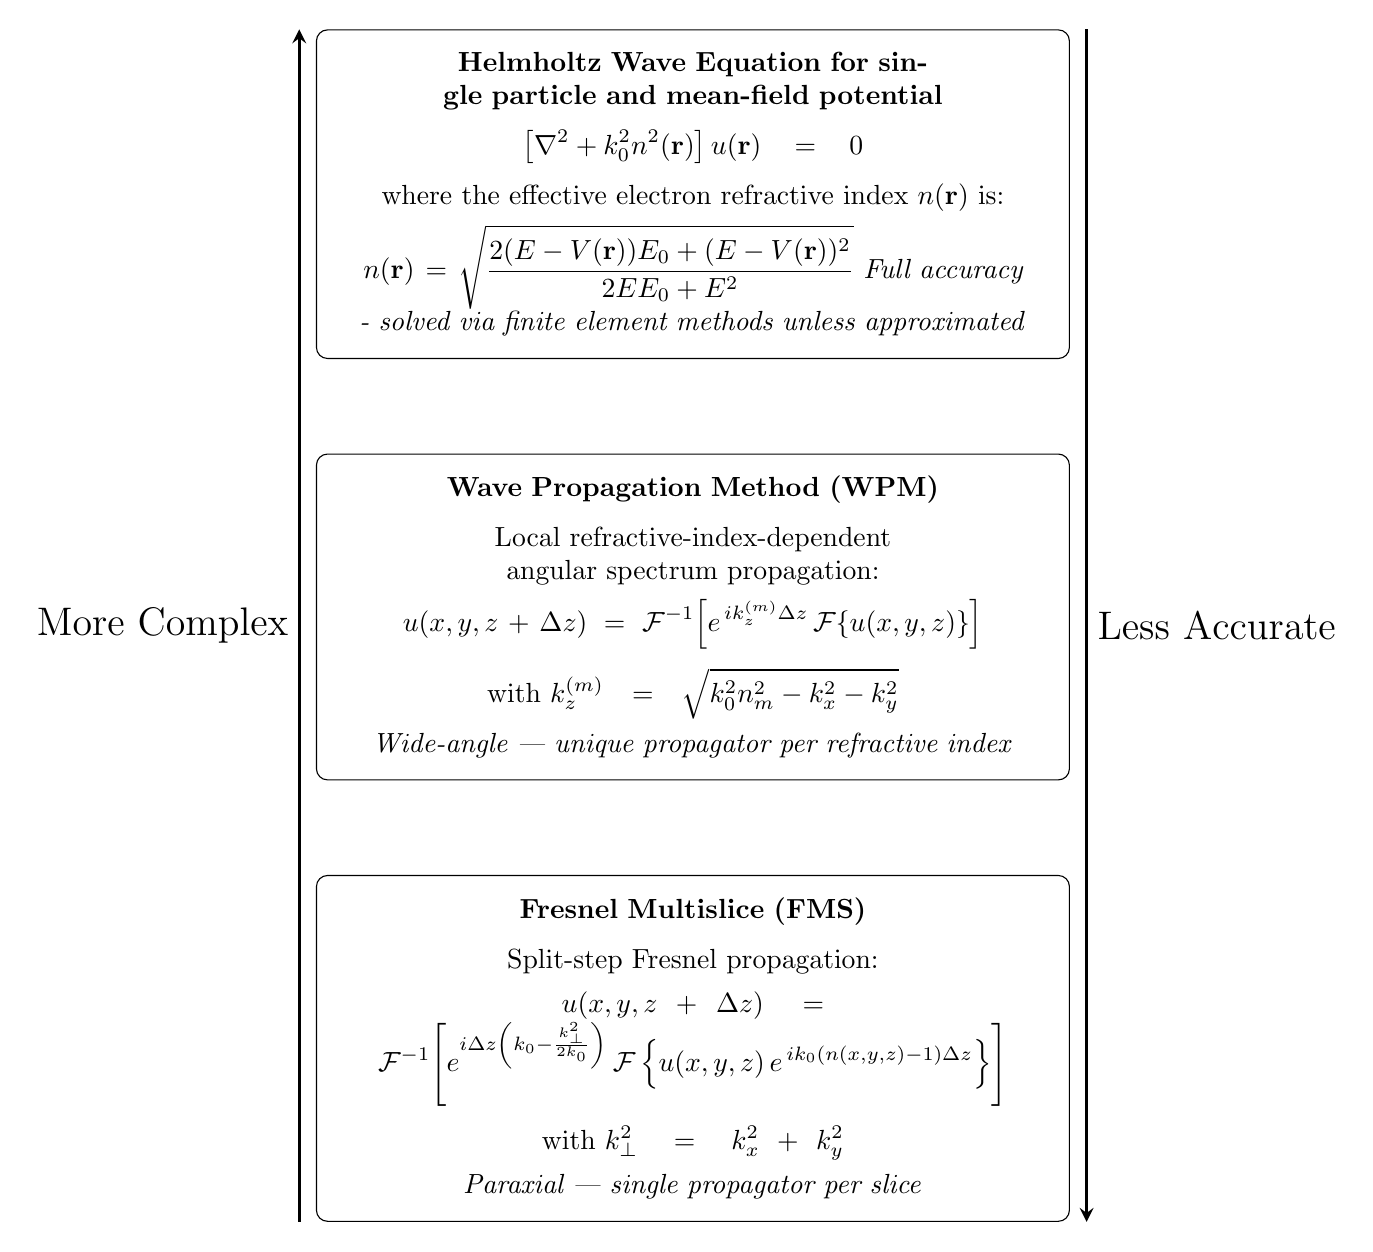
\begin{tikzpicture}[
      node distance=1.2cm,
      box/.style={
        rectangle, draw, rounded corners,
        align=center,
        text width=9cm,
        minimum height=1.25cm
      }
    ]

    % Top node: Schr -> Helmholtz via effective refractive index
    \node[box, inner sep=8pt] (helm) {%
        \textbf{Helmholtz Wave Equation for single particle and mean-field potential}\\[6pt]
        $\displaystyle \left[\nabla^2 + k_0^2 n^2(\mathbf r)\right] u(\mathbf r) = 0$\\[6pt]
        where the effective electron refractive index $n(\mathbf r)$ is:\\[4pt]
        $\displaystyle n(\mathbf r)= \sqrt{ \frac{ 2(E-V(\mathbf r))E_0 + (E-V(\mathbf r))^2 }{ 2EE_0 + E^2 } }$
        \textit{Full accuracy - solved via finite element methods unless approximated}
    };

    \node[box, below=of helm, inner sep=8pt] (wpm) {%
        \textbf{Wave Propagation Method (WPM)}\\[6pt]
        Local refractive-index-dependent angular spectrum propagation:\\[4pt]
        $\displaystyle u(x,y,z+\Delta z) =
            \mathcal{F}^{-1}\!\left[
                e^{\,i k_z^{(m)}\Delta z}\,
                \mathcal{F}\{u(x,y,z)\}
            \right]$\\[6pt]
        with $\displaystyle k_z^{(m)}=\sqrt{k_0^2 n_m^2 - k_x^2 - k_y^2}$\\[4pt]
        \textit{Wide-angle --- unique propagator per refractive index}
    };

    \node[box, below=of wpm, inner sep=8pt] (msft) {%
        \textbf{Fresnel Multislice (FMS)}\\[6pt]
        Split-step Fresnel propagation:\\[4pt]
        $\displaystyle u(x,y,z+\Delta z)=
            \mathcal{F}^{-1}\!\left[
                e^{i \Delta z \left(k_0 - \frac{k_\perp^2}{2k_0}\right)}\,
                \mathcal{F}\left\{ u(x,y,z) \, e^{\,i k_0(n(x,y,z)-1)\Delta z} \right\}
            \right]$\\[6pt]
        with $\displaystyle k_\perp^2 = k_x^2 + k_y^2$\\[4pt]
        \textit{Paraxial --- single propagator per slice}
    };

    % Left and right vertical arrows (use a fixed horizontal offset so arrows run outside the boxes)
    \draw[->, very thick, >=stealth]
        ([xshift=-5cm]msft.south) -- ([xshift=-5cm]helm.north) node[midway, left]{\Large More Complex};

    \draw[->, very thick, >=stealth]
        ([xshift=5cm]helm.north) -- ([xshift=5cm]msft.south) node[midway, right]{\Large Less Accurate};
    \end{tikzpicture}
    \caption{Schematic comparison of the exact Helmholtz formulation, WPM, and Fresnel multislice, illustrating the trade-off between accuracy and computational cost.}
    \label{fig:method_summary}
\end{figure}

\section{Results}
\subsection{High-angle beam amplitude benchmark}
To verify the accuracy of our WPM multislice implementation, we recreated the simulation presented in figure 3 of \cite{RotherScheerschmidt2009},
which compares the amplitude of a central and high-angle (135 mrad) diffracted beam after propagation through a thick gold sample.
For the central beam, all methods (MS and WPM) agree. For the high-angle beam at 135 mrad, the amplitude of the diffracted MS solutions deviates from the "ground truth" ODE solution as
the thickness of the unit cell increases. The WPM solution follows the trend of the ground truth ODE solution more closely, demonstrating that the WPM is more accurate at high angles than
the traditional MS method while maintaining the efficiency and larger step size of the FFT-based multislice method (with two slices per unit cell), provided one can use a GPU for
computation of the many binned FFTs required per slice.

\begin{figure}[ht]
    \centering
    \includegraphics[width=\textwidth,keepaspectratio]{Au_beam_amplitudes}
    \caption{Recreation of figure 3 in \cite{RotherScheerschmidt2009} showing the amplitude of the central and high-angle (135 mrad) diffracted beams
             after propagation with our multislice and wave propagation methods. Plotted in green is the "ground truth" ODE solution and the multislice solution
             to the Klein-Gordon equation. In blue are the Angular Spectrum Multislice (ASMS) solution and the Wave Propagation Method (WPM) solution.}
    \label{fig:au_beam_amplitudes}
\end{figure}

\subsection{Thick-sample STEM comparison}
To test the WPM multislice method in a more realistic scenario, we performed a STEM simulation of a thick sample of gold (100 nm),
tilted at 30 degrees relative to the incident electron beam. We compare the WPM multislice method to the traditional Fresnel multislice method.
The WPM preserves high-angle scattering and reduces phase errors that appear in the Fresnel MS solution for large tilt and thickness,
leading to stronger high-angle detector signals and improved contrast in the simulated STEM images. These results emphasize that the WPM
retains the computational structure of multislice while remaining accurate in regimes where the paraxial approximation breaks down.

\section{Conclusion}
We presented a wide-angle multislice framework based on the Wave Propagation Method, derived its relationship to the paraxial Fresnel multislice propagator,
and clarified why swapping in an angular spectrum kernel does not remove the linearization inherent to multislice. By introducing a differentiable refractive-index
binning strategy, the method becomes computationally tractable while remaining suitable for gradient-based inverse problems. Benchmarks against high-angle
reference solutions and thick-sample STEM simulations indicate that WPM provides improved accuracy in regimes where the paraxial approximation fails. Future work
will focus on systematic comparisons to Padé-based wide-angle multislice schemes and integration with large-scale ptychographic reconstructions.
\end{document}
